% Straight up stealing preamble from Eli Holmes 
%%%%%%%%%%%%%%%%%%%%%%%%%%%%%%%%%%%%%%START PREAMBLE THAT IS THE SAME FOR ALL EXAMPLES
\documentclass{article}

%Required: You must have these
\usepackage{Sweave}
\usepackage{graphicx}
\usepackage{tabularx}
\usepackage{hyperref}
\usepackage{natbib}
\usepackage{pdflscape}
\usepackage{array}
\usepackage{gensymb}
%\usepackage[backend=bibtex]{biblatex}
%Strongly recommended
 %put your figures in one place
 
%you'll want these for pretty captioning
\usepackage[small]{caption}

\setkeys{Gin}{width=0.8\textwidth} %make the figs 50 perc textwidth
\setlength{\captionmargin}{30pt}
\setlength{\abovecaptionskip}{0pt}
\setlength{\belowcaptionskip}{10pt}
% manual for caption http://www.dd.chalmers.se/latex/Docs/PDF/caption.pdf

%Optional: I like to muck with my margins and spacing in ways that LaTeX frowns on
%Here's how to do that
 \topmargin -2cm     
 \oddsidemargin -0.04cm   
 \evensidemargin -0.04cm  % same as oddsidemargin but for left-hand pages
 \textwidth 16.59cm
 \textheight 22.94cm 
 %\pagestyle{empty}       % Uncomment if don't want page numbers
 \parskip 7.2pt           % sets spacing between paragraphs
 %\renewcommand{\baselinestretch}{1.5} 	% Uncomment for 1.5 spacing between lines
\parindent 0pt% sets leading space for paragraphs
\usepackage{setspace}
%\doublespacing

%Optional: I like fancy headers
\usepackage{fancyhdr}
\pagestyle{fancy}
\fancyhead[LO]{Do early phenological events constrain later phenology?}
\fancyhead[RO]{2017}
 
%%%%%%%%%%%%%%%%%%%%%%%%%%%%%%%%%%%%%%END PREAMBLE THAT IS THE SAME FOR ALL EXAMPLES

%Start of the document
\begin{document}

% \SweaveOpts{concordance=TRUE}
 \bibliographystyle{/Users/aileneettinger/citations/Bibtex/styles/nature.bst}
\title{Do early phenological events constrain later phenology?} 
\author{A.K. Ettinger, S. Gee, and E.M. Wolkovich}
%\date{\today}
\maketitle  %put the fancy title on
%\tableofcontents      %add a table of contents
%\clearpage
%%%%%%%%%%%%%%%%%%%%%%%%%%%%%%%%%%%%%%%%%%%%%%%%%%%

\section* {Goal}
\par We aim to test the extent to which previous phenological stages constrain later ones, as this is poorly understood. We plan to submit this paper as a ``brief communication" at	American Journal of Botany ("Brief Communications—Brief Communications are short (c 3000-5000 word) research articles reporting exciting, significant new findings. They include no more than 4 figures and tables, combined. Manuscripts, and their abstracts, should be organized as described for Research articles.") or a ``rapid report" at
New Phytologist.

\section*{Abstract}
\subsection*{Premise of the study}
\subsection*{Methods}
\subsection*{Key results}
\subsection*{Conclusions}
\section* {Key words}
\section* {Introduction}
\subsection* {Hypotheses}
 %\citep{wolkovich2014}
\par Hypothesis 1: Previous phenological events constrain later events; e.g., late-fruiting species set fruit late in the season because they leaf-out late  (Figure \ref{fig:hyp}).
\par Hypothesis 2: Inter-phenophase time  constrains phenology; e.g., late-fruiting species set fruit late in the season because they require longer development time (Figure \ref{fig:hyp}).
\section* {Materials and Methods}
\subsection*{Study site and focal species}
This study was conducted at the Arnold Arboretum of Harvard University, a 281-acre park in Boston, Massachusetts, established in 1872. It contains a living collection of trees, shrubs, and vines that are native to New England, as well as others from around the world. Arboreta are great resources for studies across many species, particularly in temperate areas, since they may contain a higher diversity of tree species in one location than nearby natural areas. In addition, there is often high variation in phenology in the selection of species planted in arboreta for public enjoyment. For this study, I selected 25 focal angiosperm species with varying flowering times during the growing season (Table 1). I selected up to five individuals of each species for the study, yielding a total of 118 individuals in this study.

\subsection*{Phenology data collection}

\subsection*{Statistical analyses}
To understand the extent to which previous phenological events constrain later events (hypothesis 1), we fit linear models with each phenological stage that we observed (except budburst, the earliest stage we quantified) as the response variable (i.e. species-level mean day of year of leaf-out, flowering, fruiting, or senesence).  We fit 10 different models, each with one of the previous phenological stages as the explanatory variable. R\textsuperscript{2} and \textit{p}-value for each model are shown, with solid lines representing model fit when \textit{p}<0.05 and dashed lines representing model fit when 0.05<\textit{p}<0.10. Full model results are summarized in Table 1. All analyses were conducted in R version 3.2.4.

\section* {Results}
Main messages for Sally's thesis paper
\begin{enumerate}
\item Earlier phenological stages constrain later phenology (Figures \ref{fig:focsp}, \ref{fig:latevearly}). The strongest correlations occurred between adjacent stages (e.g. leaf-out and budburst, fruiting and flowering). Senescence was the only phenological stage not well-correlated with an earlier phanological stage.
\item Inter-phenophase duration constrains reproductive phenology (flowering and fruiting time, Figure \ref{fig:inter}). Furthermore, reproductive phenology appears to be constrained by both earlier inter-phenophase times (e.g. time between flowering and budburst, time between fruiting and flowering) and later interphase times (e.g. time between senescence and flowering). However, growth phenology was not strongly constrained.

\end{enumerate}
\section* {Discussion}
These stages support hypothesis 1, these support hypothesis 2, these are intermediate
Fruiting takes about 0-20 days for most species
Expect correlations could be strongest  at biggest at end of season. Geometric constraint.
\section* {Conclusions}
Next steps: Encourage a phylogenetic approach, collect data across years. We observed variation at whole organism level- may want to explore at individual flower/fruit level. 

\section* {Tables}

\begin{table}[p]
  \caption{\textbf{Focal species.} Twenty-five angiosperm species were selected, based on their flowering phenology. The number of individuals of each species observed at the Arnold Arboretum from spring through fall 2015 is in parentheses.}
\begin{footnotesize} 
   \begin{tabular}{| p{5.5cm} | p{5.5cm} | p{5.5cm} |}
    \hline
  \bf{Early season flowering} & \bf{Mid season flowering} & \bf{Late season flowering} \\ \hline
    \textit{Aesculus flava} (5) & \textit{Carya glabra} (5) & \textit{Catalpa speciosa} (5) \\ 
    \textit{Betula alleghaniensis} (5) & \textit{Carya ovata} (5) & \textit{Kalopanax septemlobus} (3) \\ 
    \textit{Betula nigra} (5) & \textit{Crataegus crus-galli} (5) & \textit{Styphnolobium japonicum} (5) \\ 
\textit{Gleditsia triancanthos} (5) & \textit{Fagus engleriana} (4) & \textit{Tilia americana} (5) \\ 
\textit{Liriodendron tulipifera} (5) & \textit{Fagus grandifolia} (5) & \textit{Tilia japonica} (5) \\ 
\textit{Phellodendron amurense} var. \textit{lavallei} (4) & \textit{Fraxinus chinensis} (5) &\\ \textit{Populus deltoids} ssp. \textit{deltoids} (5) & \textit{Liquidambar styraciflua} (5) & \\ 
\textit{Pyrus calleryana} var. \textit{dimorphophylla} (3) & \textit{Platanus occidentalis} (5) & \\ 
\textit{Pyrus ussuriensis} var. \textit{hondoensis} (5) & \textit{Quercus glandulifera} (4) & \\ \textit{Quercus alba} (5) & \textit{Quercus rubra} (5) &  \\ \hline
     \end{tabular}    
\end{footnotesize} 
    \end{table}
\clearpage

\section* {Figures}
\begin{figure}[p]
  \centering
  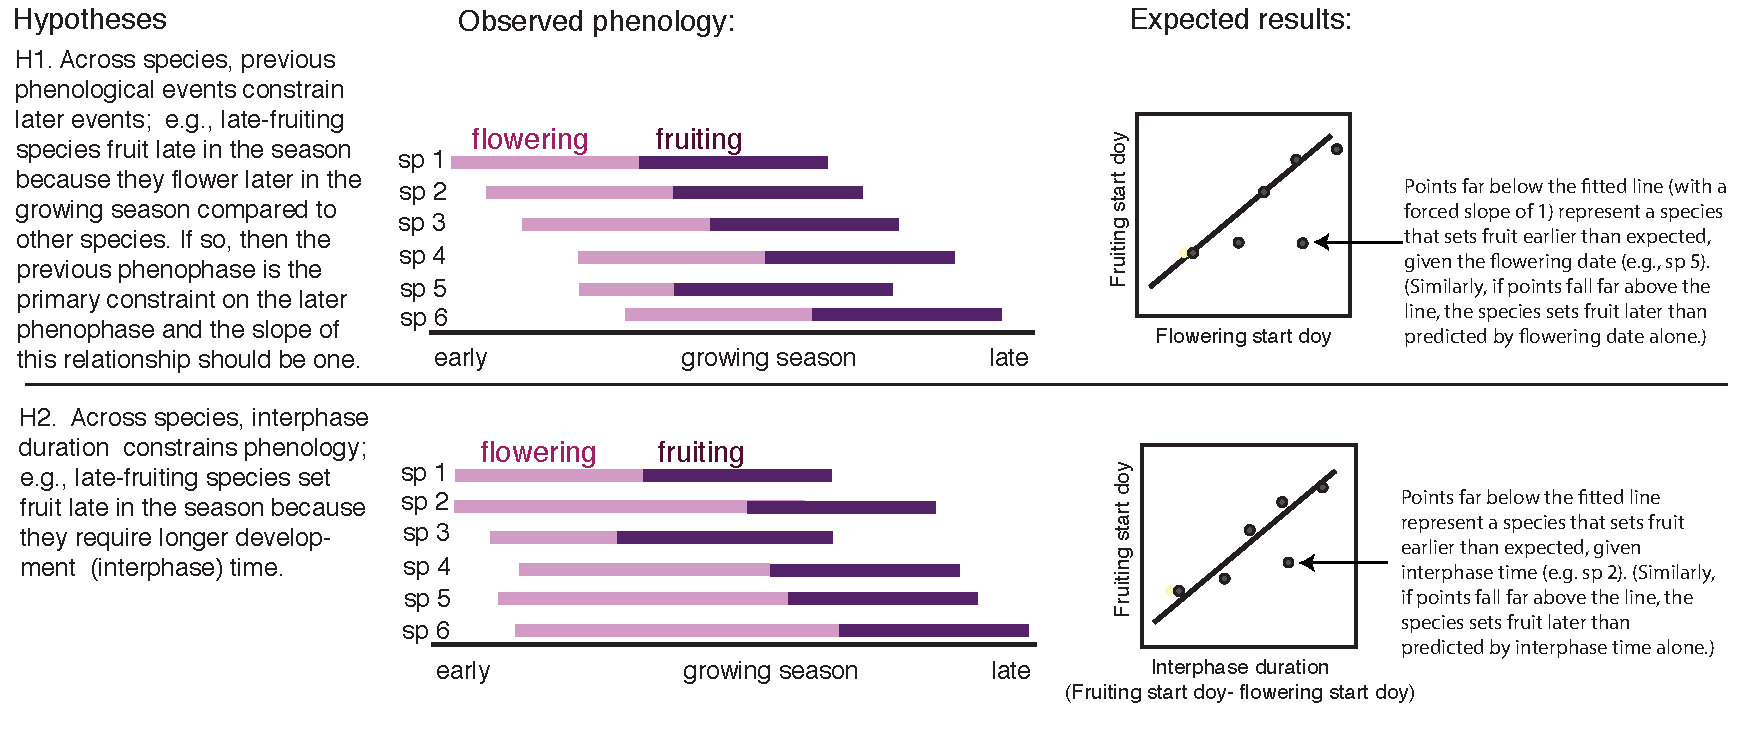
\includegraphics{../analyses/figures/hypotheses3.pdf} 
  \caption{\textbf{Hypotheses.} We show flowering and fruiting as examples of consecutive phenological events. We expected the same patterns for other consecutive events,such as leaf bud-burst and leaf-out. Inter-phenophase duration is the time between phenological events, e.g., the number of days between the start of flowering and the start of fruiting.} 
 \label{fig:hyp}
\end{figure}
 
\begin{figure}[h]
  \centering
  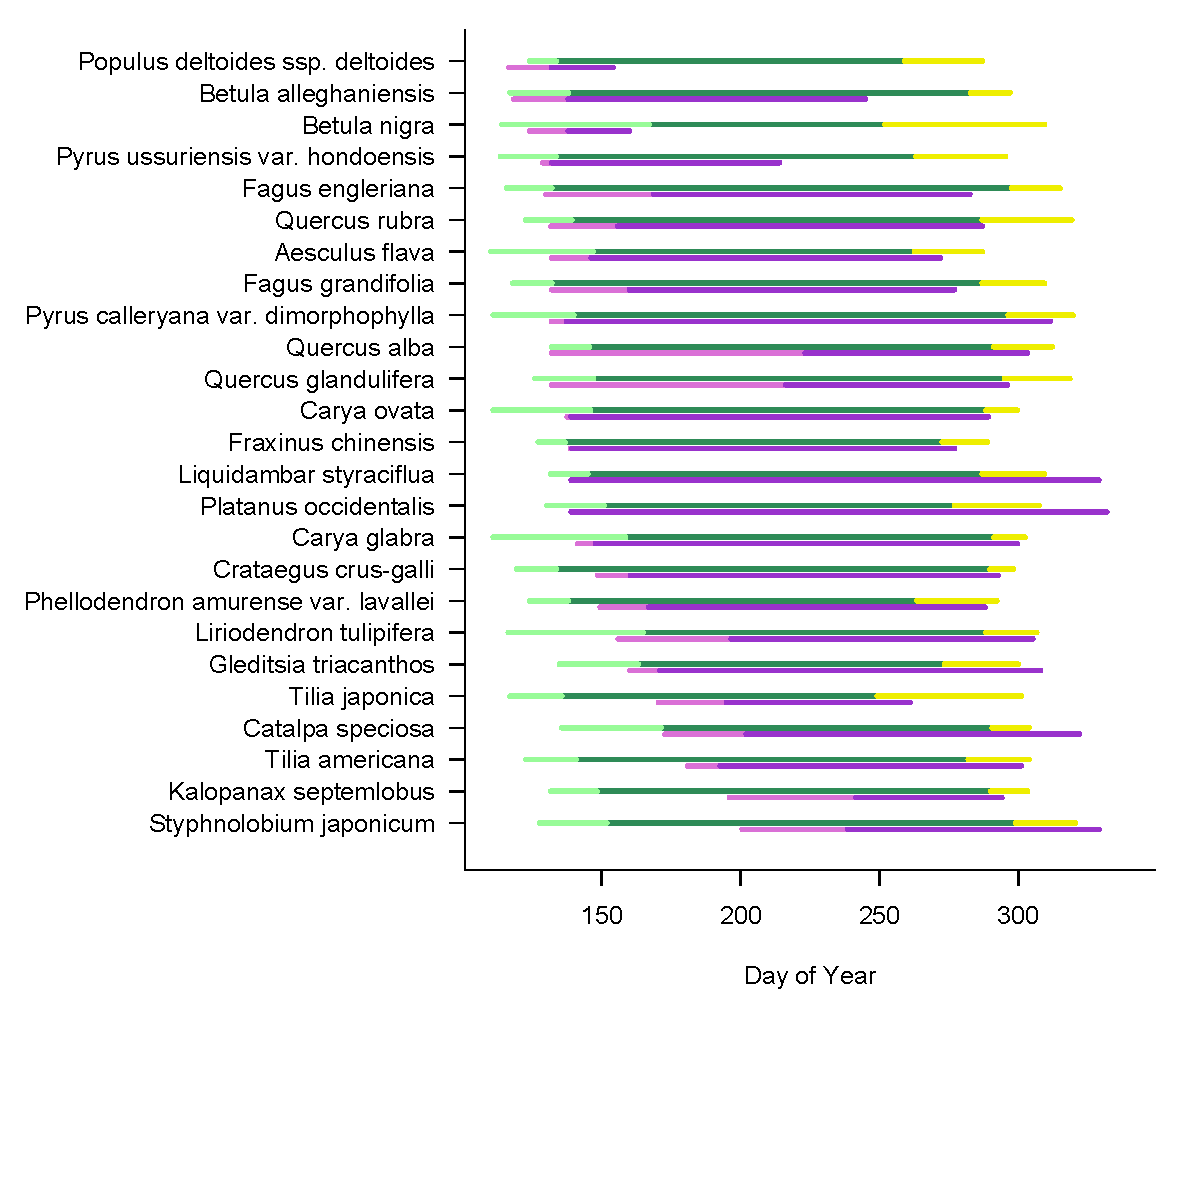
\includegraphics{../analyses/figures/grosea_repsort.pdf}
  \caption{\textbf{Focal species' phenology during the 2015 growing season, sorted by their mean first-flower dates.} For growth phenology, light green represents the bud-burst phase (from its mean start day-of-year to the mean start day-of-year for leaf-out, across all individuals within a species), dark green represents full leaf-out (from the mean day-of-year when fully-expanded leaves were first observed through the start of senescence), and yellow represents the senescence phase (from the mean day-of-year when leaves first began changing color through the mean day-of-year when more than 95 percent of leaves on the tree had changed color). For reproductive phenology, light purple represents the flowering phase (from the mean day-of-year when flowers first appeared to the mean day-of-year when fruits first appeared, across all individuals within a species) and dark purple represents the fruiting phase (from the mean day-of-year when fruits first appeared to the mean day-of-year when more than 95 percent of fruits were first observed as ripe). Species are ordered from early to late first flower dates.}
  \label{fig:focsp}
\end{figure}
  
  \begin{figure}[h]
  \centering
  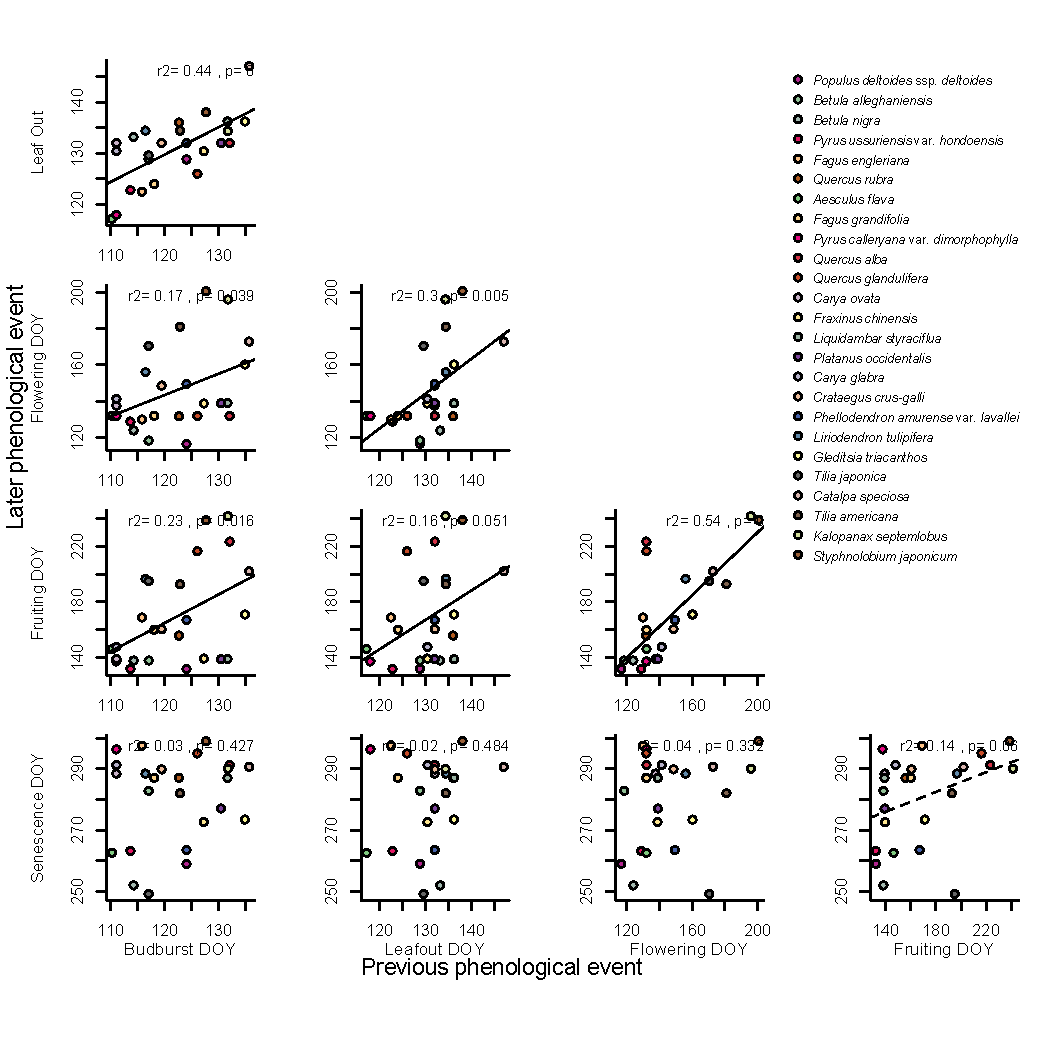
\includegraphics{../analyses/figures/latevearly_rp_col_legend.pdf}
  
  \caption{\textbf{Relationships among phenological stages across the 25 focal species.} Linear models were fit with the species-level mean day of year of the later phenological stages as the response variable, and mean day of year of earlier stage as the explanatory variable. R\textsuperscript{2} and \textit{p}-value for each model are shown, with solid lines representing model fit when \textit{p}<0.05 and dashed lines representing model fit when 0.05<\textit{p}<0.10. Full model results are summarized in Table 2.Species in the legend are ordered from early to late first flower dates, as in Figure 2.}
  \label{fig:latevearly}
\end{figure}
\begin{figure}[h]
  \centering
  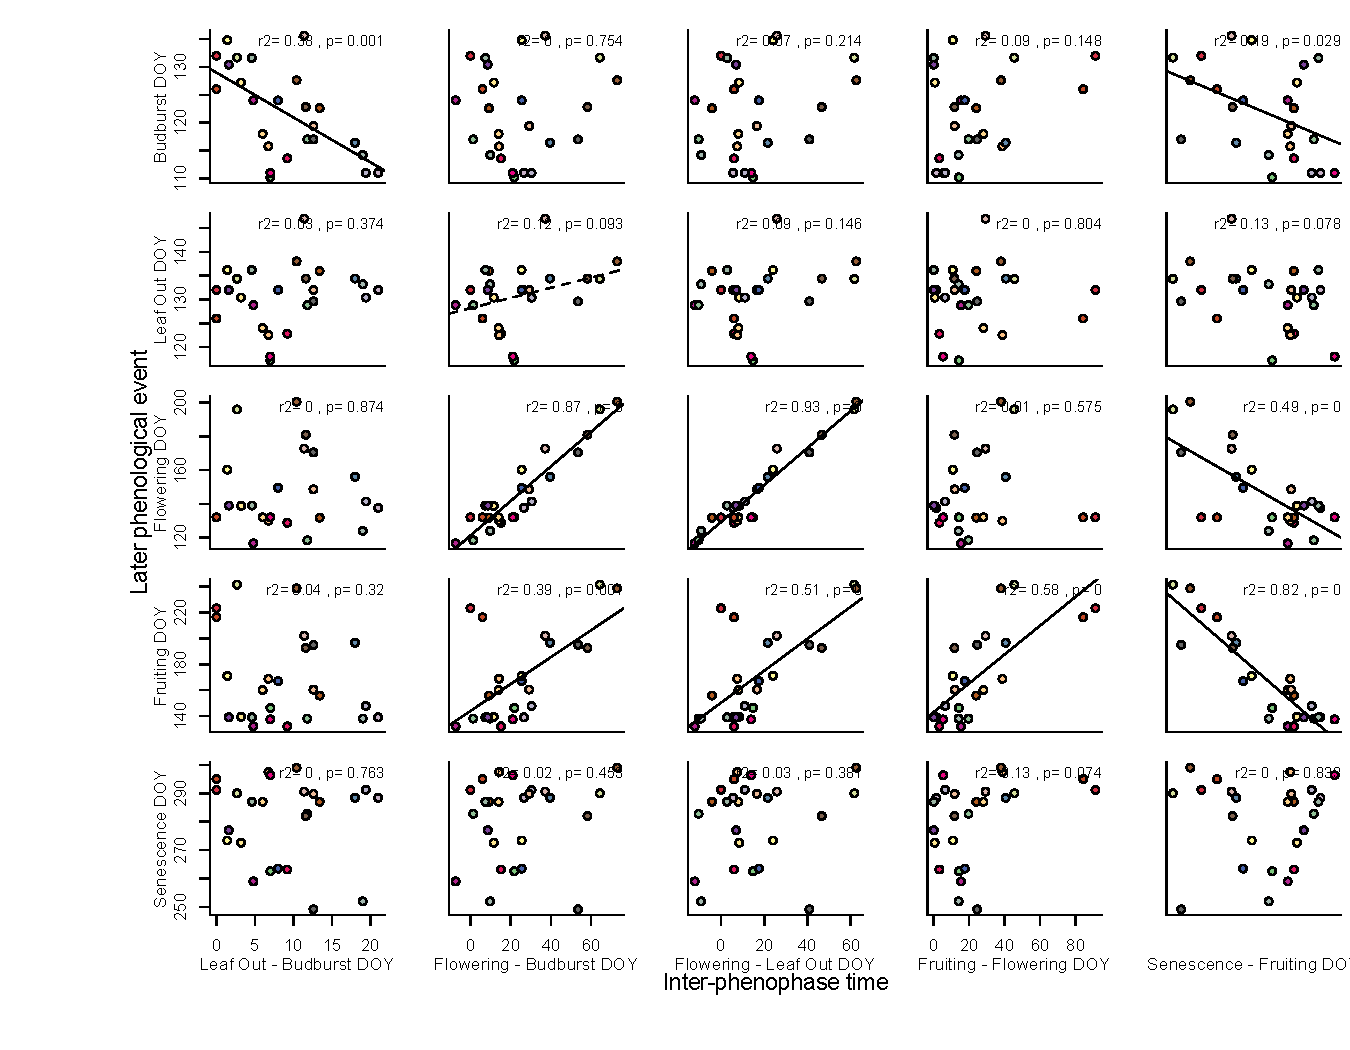
\includegraphics{../analyses/figures/adj_stagesmegaplot_col2.pdf}
  \caption{\textbf{Relationships among phenological stages and inter-phenophase duration across the 25 focal species.} Inter-phenophase duration is the time between the start of the earlier phenological event and the start of the later phenological event, e.g., the number of days between the species' mean start of flowering and its mean start of fruiting. Linear models were fit with the species-level mean day of year of the later phenological stages as the response variable, and interphenophase duration as the explanatory variable. R\textsuperscript{2} and \textit{p}-value for each model are shown, with solid lines representing model fit when \textit{p}<0.05 and dashed lines representing model fit when 0.05<\textit{p}<0.10.Full model results are summarized in Table 3.}
  \label{fig:inter}
   \end{figure}

%%%%%%%%%%%%%%%%%%%%%%%%%%%%%%%%%%%%%%%%
\end{document}
%%%%%%%%%%%%%%%%%%%%%%%%%%%%%%%%%%%%%%%%
